\documentclass[conference]{IEEEtran}
\usepackage{times}
\usepackage{graphicx}
\usepackage{tikz}
\usepackage{mathtools, amsfonts, breqn, subcaption}
\usepackage{tabu}
\DeclareMathOperator*{\argmin}{arg\,min}

% numbers option provides compact numerical references in the text. 
\usepackage[numbers]{natbib}
\usepackage{multicol}
\usepackage[bookmarks=true]{hyperref}

\pdfinfo{
   /Author (Varun Murali)
   /Title  (Evaluation of Safe Control Policies for Mobile Robots in Dynamic Environments)
   /CreationDate (D:20101201120000)
   /Subject (Safe Robotics)
   /Keywords (Safety Control)
}

\begin{document}

% paper title
\title{Evaluation of Safe Control Policies for \\Mobile Robots in Dynamic Environments }

% You will get a Paper-ID when submitting a pdf file to the conference system
\author{Varun~Murali, Niharika~Arora, Ian~Buckley}

%\author{\authorblockN{Michael Shell}
%\authorblockA{School of Electrical and\\Computer Engineering\\
%Georgia Institute of Technology\\
%Atlanta, Georgia 30332--0250\\
%Email: mshell@ece.gatech.edu}
%\and
%\authorblockN{Homer Simpson}
%\authorblockA{Twentieth Century Fox\\
%Springfield, USA\\
%Email: homer@thesimpsons.com}
%\and
%\authorblockN{James Kirk\\ and Montgomery Scott}
%\authorblockA{Starfleet Academy\\
%San Francisco, California 96678-2391\\
%Telephone: (800) 555--1212\\
%Fax: (888) 555--1212}}


% avoiding spaces at the end of the author lines is not a problem with
% conference papers because we don't use \thanks or \IEEEmembership


% for over three affiliations, or if they all won't fit within the width
% of the page, use this alternative format:
% 
%\author{\authorblockN{Michael Shell\authorrefmark{1},
%Homer Simpson\authorrefmark{2},
%James Kirk\authorrefmark{3}, 
%Montgomery Scott\authorrefmark{3} and
%Eldon Tyrell\authorrefmark{4}}
%\authorblockA{\authorrefmark{1}School of Electrical and Computer Engineering\\
%Georgia Institute of Technology,
%Atlanta, Georgia 30332--0250\\ Email: mshell@ece.gatech.edu}
%\authorblockA{\authorrefmark{2}Twentieth Century Fox, Springfield, USA\\
%Email: homer@thesimpsons.com}
%\authorblockA{\authorrefmark{3}Starfleet Academy, San Francisco, California 96678-2391\\
%Telephone: (800) 555--1212, Fax: (888) 555--1212}
%\authorblockA{\authorrefmark{4}Tyrell Inc., 123 Replicant Street, Los Angeles, California 90210--4321}}


\maketitle

\begin{abstract}
With the growth of domestic robot industry, it is important to understand the navigation of mobile robots in dynamic environments. With increased interaction between humans and robots, and an increasingly shared workspace, it is important to study the safety of the robotic system and the extent of guarantees that can be made to minimize risk of injury. We present a nonlinear control approach to the navigation problem that achieves the objective of reaching pre-defined locations with provable guarantees of safety. Verification of the controller is performed first in MATLAB simulation, which shows that the controller is capable of driving the system to a pre-defined location while maintaining all required safety rules defined in it's environment. The controller is then implemented in the ROS framework, first in Gazebo simulation to corroborate the MATLAB results, and then on the Segway RMP 200 based mobile robot \textit{Jeeves}, demonstrating that the nonlinear navigation controller successfully traverses the gap between theory and practice. 
\end{abstract}

\IEEEpeerreviewmaketitle

\section{Introduction}
Safety is an important concern for mobile robots working in collaborative environments. Typical robotic systems separately deal with safety and task completion in a hierarchical fashion--a high level controller decides which control law to use based on the situation. Navigation is of fundamental concern for mobile robots. The ability to successfully avoid obstacles, both static and dynamic, while moving towards a goal location largely determines the utility of a mobile robotic platform. It is critical that robots avoid obstacles for their own safety as well as the safety of the people around them. We use the navigation problem to motivate the direct addition of safety into the controller for the robot.

After formulating the navigation control strategy, MATLAB simulation is used to verify that the navigation control strategy safely drives the state of the robot to a target. After thoroughly substantiating the efficacy of the navigation control strategy in MATLAB simulation, the controller is implemented in the ROS framework and evaluated in both Gazebo simulation and on the Segway RMP 200 based mobile robot \textit{Jeeves}, verifying the navigation control strategy in a real world scenario.

\section{Approach}
Control Lyapunov functions and control barrier functions are formulated to individually accomplish the objectives of navigation and obstacle avoidance. As in \cite{amesACC} and \cite{ames2014esclf}, the control Lyapunov and barrier functions are soft and hard constrained in a Quadratic Programming based controller to achieve safe navigation. Figure~\ref{fig:obs} shows the egocentric coordinate system of the robot and describes the variables used in the polar form of the unicycle dynamics modelling the robot, given by: 
\begin{equation}
\left(
\begin{matrix}
\dot{r}\\
\dot{\theta}\\
\end{matrix}
\right)
=
\left(
\begin{matrix}
- v \text{ cos}(\delta)\\
\frac{v}{r} \text{ sin}(\delta)\\
\end{matrix}
\right)
\end{equation}
\begin{equation}
\dot{\delta}=\frac{v}{r} \text{ sin}(\delta)+\omega.
\end{equation}
\begin{figure}[t]
\begin{center}
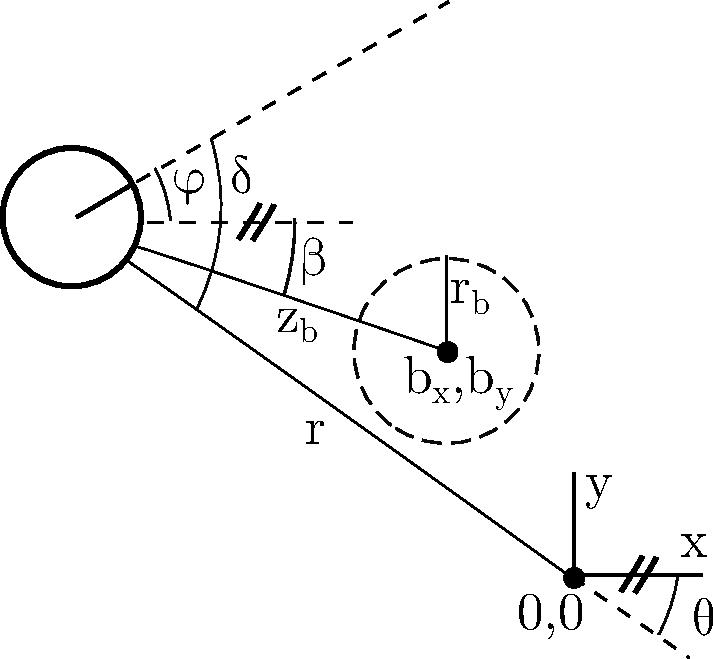
\includegraphics[scale=0.35]{obs.pdf} 
\caption{The egocentric co-ordinate system of the robot is shown above. $r$ is the radial distance of the robot from the origin, $\phi$ is the heading of the robot in the target frame, $\theta$ is the orientation of the target frame in the robot frame, and $\delta$ is  the egocentric heading. $z_b$ is the vector joining the center of the robot to the obstacle,  $r_b$ is the minimum safe distance from the obstacle, and $\beta$ is the angle between the global $x$-axis and $z_b$. \label{fig:obs}} 
\end{center}
\end{figure}

\subsection{Control Lyapunov Functions}
To design the navigation control law, two control Lyapunov functions are formulated. The standard quadratic Lyapunov function candidate is first considered:
\begin{equation}
V_1=\frac{1}{2}(r^2+\theta^2)=-r v \text{ cos}(\delta) + \theta v \text{ sin}(\delta)\label{v1}
\end{equation}
%\begin{align}
%V_1&=\frac{1}{2}(r^2+\theta^2)\label{v1}\\
%&=-r v \text{ cos}(\delta) + \theta v \text{ sin}(\delta)
%\end{align}
Fixing $\delta = \text{arctan}(-k_1\theta)$ to enforce a virtual steering control as in \cite{park2011}, the derivative of the Lyapunov function becomes:
\begin{equation}
\dot{V_1}=-r v \text{ cos}(\text{arctan}(-k_1\theta)) + \theta v \text{ sin}(\text{arctan}(-k_1\theta)).
\end{equation} 

Because $\theta\in (-\pi,\pi]$, $v>0$, and $r\geq 0$ , $\dot{V}<0$ $\forall \theta$, $r\neq0$; thus, the steering control asymptotically drives $r,\theta\to 0$. By choosing $v=k_3 r$ in some neighborhood of $r=0$ for positive constant $k_3,$ the singularity at $r=0$ is removed and the system is globally asymptotically stable.  

To drive the state to zero through the steering control, the heading must be driven such that $\delta = \text{arctan}(-k_1\theta).$ An objective $z_1$ is defined: 
\begin{equation}
z_1 \equiv \delta - \text{arctan}(-k_1\theta).
\label{z1}
\end{equation} The derivative is calculated to yield:
\begin{equation}
\dot{z_1}=\left( 1+\frac{k_1}{1+(k_1\theta)^2}\right) \frac{v}{r}\text{ sin}(z_1+\text{ arctan}(-k_1\theta))+\omega.
\end{equation}
Feedback linearization can be used to achieve this objective by choosing the angular velocity 
\begin{equation}
\begin{split}
\omega = -\frac{v}{r}\left[ k_2 z_1+\left( 1 + \frac{k_1}{1+(k_1\theta)^2} \right)\right.\\
\left. \vphantom{\frac{v}{r}} \text{sin}(z_1+\text{ arctan}(-k_1\theta))\right],
\end{split}
\end{equation}
the objective dynamics are globally exponentially stable with the following form: $\dot{z_1}=-k_2(v/r)z_1,$ where $k_1$ and $k_2$ can be chosen to increase or decrease how aggressive the steering control is.

A second steering controller is designed to drive the state away from the origin and is defined by the following objective: \begin{equation}z_2=\delta-\text{ atan}(k_1\beta).\label{z2}\end{equation}
The derivative of $z_2$ is similarly computed as with $z_1$, and is given by $\dot{z_2} = \dot{\delta}.$ The steering objectives are modelled along with other constraints by defining: 
\begin{equation} V_2 = \frac{1}{2}  z_*^2, \label{v2}\end{equation}
where $z_*$ represents the objectives $z_1$ and $z_2$ in \eqref{z1} and \eqref{z2}.

Feedback linearization can be used to show that steering control is achieved; thus, there exist control inputs that satisfy the control Lyapunov function $\dot{V_2}<0$; furthermore, following Definition 3 in \cite{ames2014esclf}, a control Lyapunov function is exponentially stabilizing if it satisfies
\begin{equation}
\inf_{u\in U}\left[ \dot{V}+\gamma V \right] \leq 0
\label{eq:esclf}
\end{equation}
for some constant $\gamma >0$, so choosing the correct inputs $u$ will achieve the desired exponential stabilization. 

\subsection{Control Barrier Functions}
Two control barrier functions are formulated to keep the robot in the safe set $C$ defined by:
\begin{align}
C &= \left\lbrace x \in \mathbb{R}^3 | z_b\geq r_b\right\rbrace\\
\partial C &= \left\lbrace x \in \mathbb{R}^3 | z_b=r_b\right\rbrace\\
\text{Int}(C) &= \left\lbrace x \in \mathbb{R}^3 | z_b > r_b\right\rbrace.
\end{align}

As presented in \cite{ames2015robust}, a barrier function is a zeroing barrier function $h(x)$ if $\dot{h}(x)\leq \gamma h(x).$ For the purpose of avoiding obstacles in the event that the robot leaves the safe set, a zeroing barrier function was chosen with the following form:
\begin{equation}
h(x)=\sqrt{(-v\text{ cos}(\theta)-b_x)^2+(v\text{ sin}(\theta)-b_y)^2}.
\end{equation}
The derivative of $h(x)$ is given by the following expression:
\begin{equation}
\begin{split}
\dot{h}(x)=\frac{1}{h(x)} \left[ (-v\text{ cos}(\delta)(r-b_y\text{ sin}(\theta)+b_x\text{ cos}(\theta)) \right. \\
\left. \vphantom{\frac{1}{h(x)}}-v\text{ sin}(\delta)(b_x\text{ sin}(\theta)+b_y\text{ cos}(\theta))\right]
\end{split}
\label{zbf}
\end{equation}

A second barrier function was chosen to prevent the robot from leaving the safe set. According to Definition 2 in \cite{amesACC}, the barrier function $B$ is a control barrier function if 
\begin{equation}
\inf_{u\in U}\left[ \dot{B}+\frac{\gamma}{B} \right] \leq 0.
\label{eq:cbf}
\end{equation}
Thus, by satisfying the equation $\dot{B}\leq 1/B$, the barrier function will prevent the robot from leaving the safe set. The barrier function was chosen to be
\begin{equation}
B=\frac{1}{h(x)-z_{safe}},
\label{bf}
\end{equation}
and its derivative is given by
\begin{equation}
\dot{B}=\frac{-\dot{h}(x)}{(h(x)-z_{safe})^2}.
\end{equation}

%TODO check constraints
\subsection{QP Based Controller}
Quadratic programming is used to find control inputs that simultaneously satisfy both the soft and hard constraints of the system. To minimize control inputs, the cost function $\textbf{u}^TH\textbf{u}+F^T\textbf{u}$ is chosen. The QP is given by the following expression:
\begin{equation}
u^*(x,z) = \argmin_{\textbf{u}=
\left[\begin{matrix}
v\\
\omega\\
\lambda_1\\
\lambda_2\\
\alpha_1\\
\alpha_2
\end{matrix}\right]
\in \mathbb{R}^6}
\frac{1}{2}\textbf{u}^TH\textbf{u}+F^T\textbf{u} 
\label{QP}
\end{equation}
\begin{align}
\text{ s.t.\hspace{1cm}}
\dot{V_1} -\alpha_1 V_1 & \leq\lambda_1\\
\dot{V_2} -\alpha_2 V_2 & \leq\lambda_2\\
\dot{h(x)}-\alpha_1 h(x) & \leq \lambda_1\\
\dot{B} & \leq \gamma/B\\
c_a \leq v & \leq c_b\\
c_c\leq \omega & \leq c_d\\
\alpha_1,\alpha_2 & \leq 0
\end{align}

In \eqref{QP}, the sparse matrix $H\in \mathbb{R}^{6\times 6}$ has 1 in the first four elements of the diagonal, and the last two elements of the sparse vector $F^T\in \mathbb{R}^{1\times 6}$ are 10 and 1. The last two elements in the diagonal of $H$ were chosen to be zero to ensure that the negative quadratic cost of the variables $\alpha_1$ and $\alpha_2$ is as large as possible. Conversely, the last two elements of $F^T$ were chosen to ensure that $\alpha_1$ and $\alpha_2$ were negative to minimize the cost. The slack variables $\lambda_1$ and $\lambda_2$ are used to create soft constraints on the control Lyapunov functions and the zeroing control barrier function, and $c_{a-d}$ are actuation constraints on the linear and angular velocities of the robot.

The control Lyapunov functions $V_1$ and $V_2$ are the Lyapunov functions corresponding to the objectives of driving the state to zero and enforcing the steering control respectively; the equations are given by \eqref{v1} and \eqref{v2}. Because there are two steering objectives, $z_1$ in \eqref{z1} and $z_2$ in \eqref{z2}, for $V_2$, two QP control laws are required: one which drives the state towards the target while avoiding obstacles, and the other that drives the state in such a way that the robot steers away from obstacles. Toggling between steering objectives is dependent on the obstacle measurement. If the robot is not in $C$ (e.g. $z_b\leq r_b$), then the steering objective $z_2$ is used. Otherwise, $z_1$ is used, and $\alpha_1=0$ is additionally enforced. $h(x)$ and $B$ in the QP controller are given in equations \eqref{zbf} and \eqref{bf}. 

\section{Results}
MATLAB simulation was used to verify that the navigation control strategy enabled the robot to navigate to the desired position while avoiding obstacles. Figure~\ref{fig:octoplot} shows that the navigation control strategy is capable of driving the robot to the final position while avoiding obstacles.

\begin{figure}[t]
\begin{center}
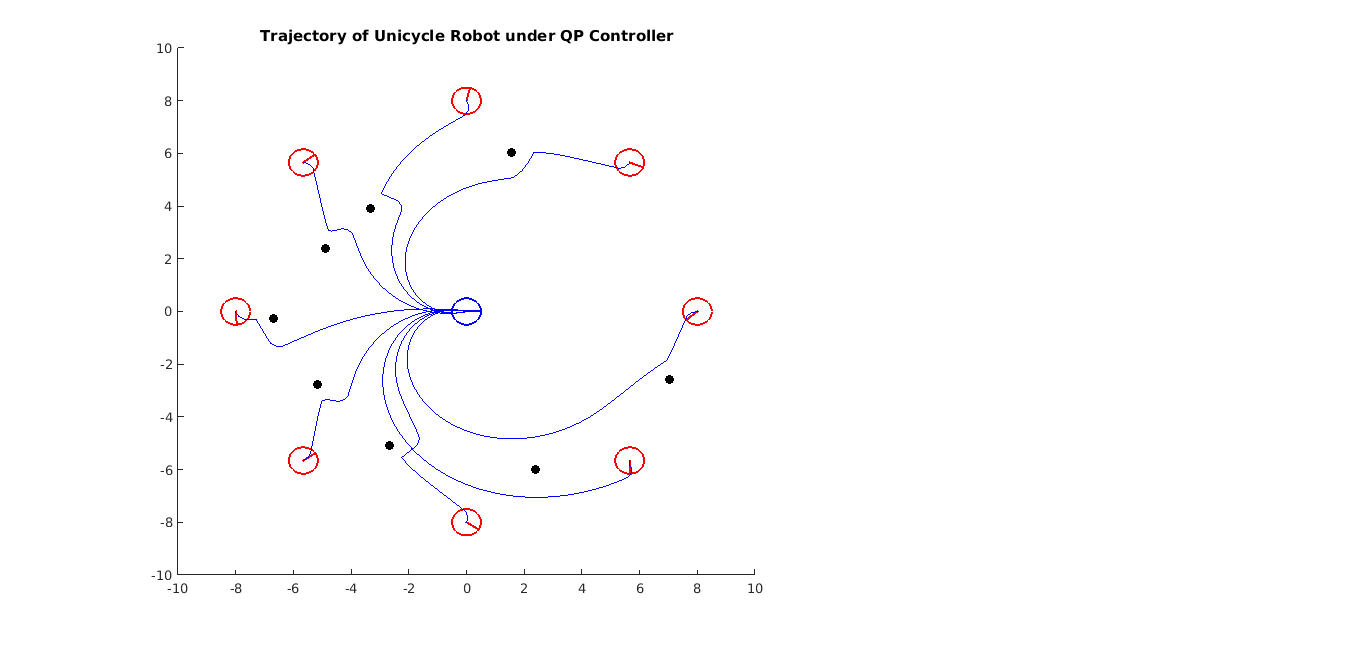
\includegraphics[scale=0.3]{octoPlotProofEditSqur.png} 
\caption{The figure above shows the same initializations at eight different starting locations and the trajectories followed by the robot to the origin to show that the robot can generate a trajectory from an arbitrary initial condition to the origin while avoiding the obstacle.\label{fig:octoplot}}
\end{center}
\end{figure}

\begin{figure}[b]
\centering
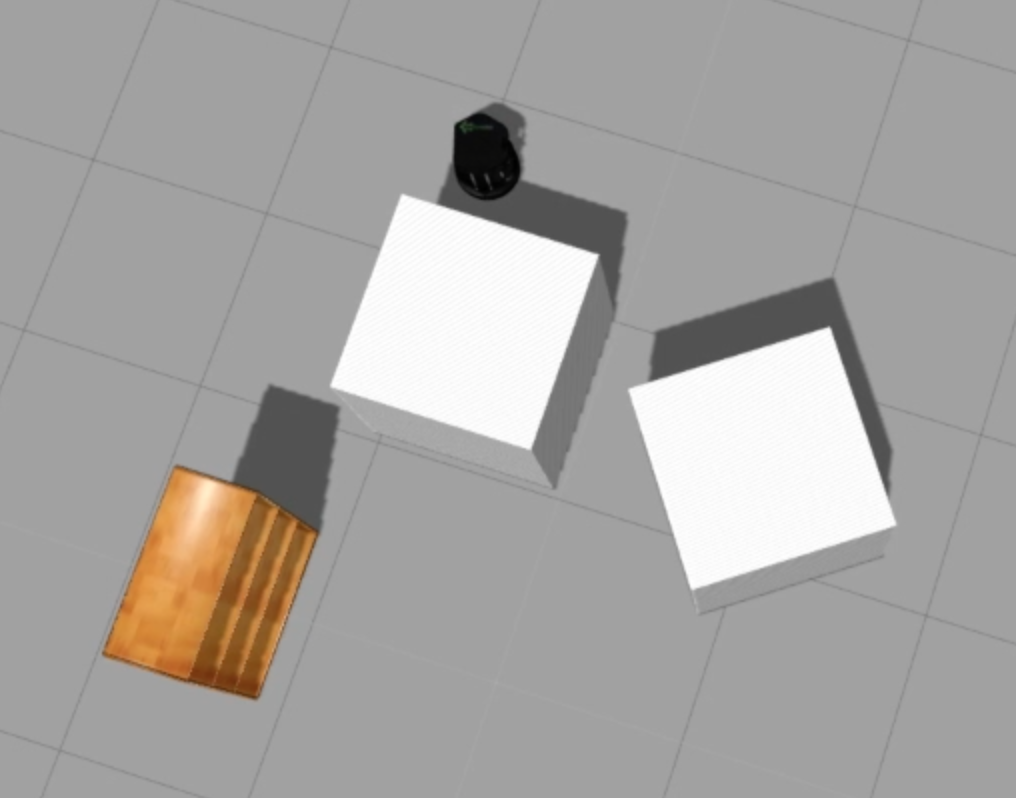
\includegraphics[scale=0.3]{Gazebo_exp.png} 
\caption{Gazebo simulation of a robot using the naviagtion control strategy shows that the robot is able to navigate to the target location while safely avoiding obstacles in its path\label{fig:gazebo}}
\end{figure}

Implementing the navigation control law in the ROS framework, Gazebo simulation, shown in Figure~\ref{fig:gazebo}, was used to corroborate the results of the MATLAB simulation. Following success in Gazebo, robot experiments were performed on the Segway robot \textit{Jeeves}. The robot is commanded to drive to a set point and the optimal $u$ is computed at every time step. The dynamics are propagated forward using the odometry. Acting as a dynamic obstacle, a human moved within the minimum permissible safe obstacle distance, and as can be seen in Figure \ref{fig:jeeves_exp}, the robot did not violate the safety constraints. An experimental run can be seen at \url {https://youtu.be/uhTiYyZxtfc}. The video shows that the robot maintains its safe distance from the human and attempts to avoid the human--when the human leaves the radius of influence, the robot is free navigate.

\begin{figure}[t]
\centering
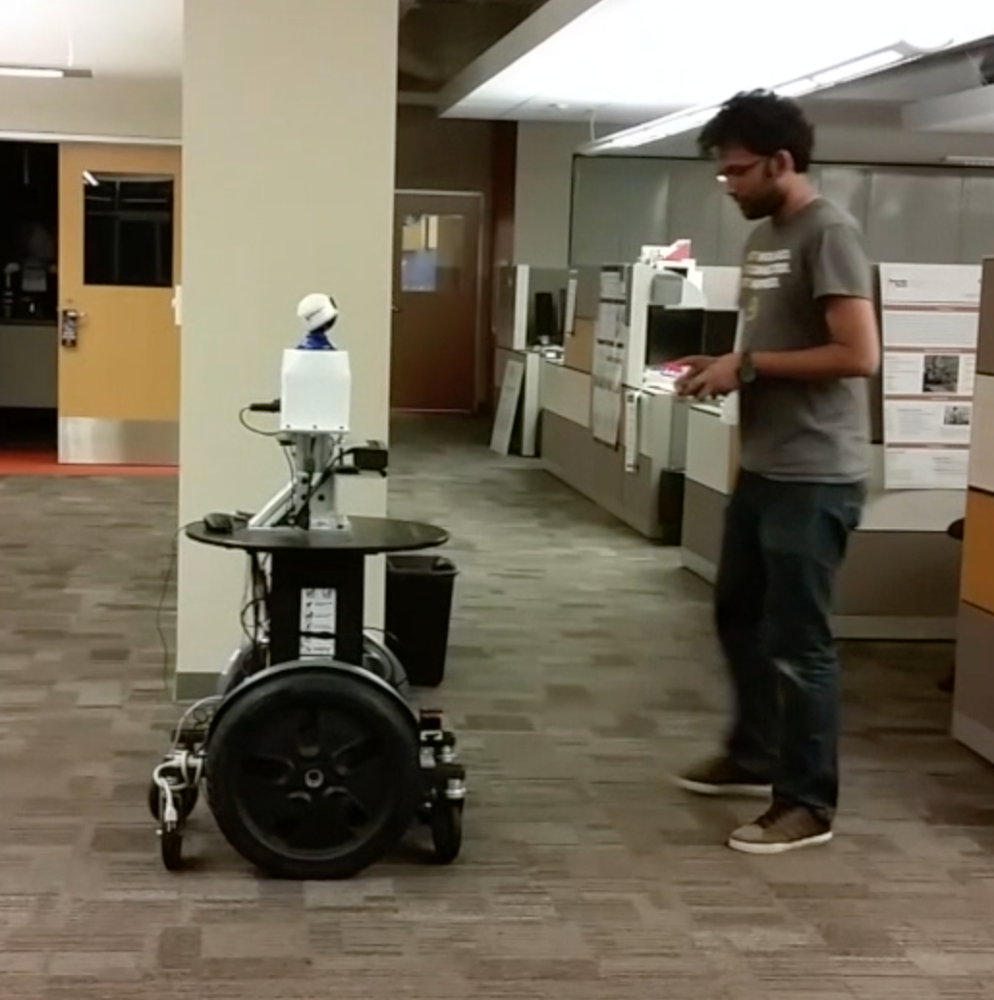
\includegraphics[scale=0.13]{jeeves_exp.png} 
\caption{Robot experiment with the Segway RMP robot \textit{Jeeves}. The robot is stopped at a safe distance from the human. \label{fig:jeeves_exp}}
\end{figure}


\section{Conclusion}
With MATLAB and Gazebo simulation and implementation on the \textit{Jeeves} platform, we show that the nonlinear controller is generalizable to multiple robots. The theoretical analysis shows that the QP based controller stabilizes the system while satisfying safety constraints. The experimental results show that the system can be implemented on a real world system and demonstrate that the results are consistent with the claims. Future work will consider the use of different barriers for different obstacles with particular emphasis on human-robot interaction--determining acceptable distances from humans will enable safe navigation in a socially acceptable manner.

\bibliographystyle{plainnat}
\bibliography {bibi}



%% Use plainnat to work nicely with natbib. 




\end{document}


